% Chapter 1

\chapter{TDSE Solutions for Time-Dependent Potentials} % Main chapter title

\label{Chapter4} % For referencing the chapter elsewhere, use \ref{Chapter1} 

%----------------------------------------------------------------------------------------
\section{Qualitative Expectation for Results}
Previously we saw that solutions to the TISE can be expressed as weighted sums of bound eigenstates, where each bound eigenstate corresponds to a distinct energy. It was also shown that if no external potential acts on the system these weights will not change as the wavefunction evolves with time; we used this fact to measure the accuracy of our propagators in the previous chapter. 

The fact that these weights remain constant with no external potential being applied is equivalent to saying that the energy of the system remains constant under time evolution; this makes physical sense as a statement of the conservation of energy. When an external field is applied, the system will either gain or lose energy over time - and so these weights will change during time evolution. 

As the weight / coefficient of each eigenstate corresponds to the probability of the system being in that state, by constructing appropriate time-dependent external potentials we can model how the probabilities of the system being in particular eigenstates changes in the event of some physical interactions; for example absorbing a laser pulse. 

The rest of this chapter consists of investigating how the system, initially in the Ground State, evolves under the influence of different simulated interactions - by investigating the change to the Ground State population under the interactions over time.

\section{Linearly Increasing Potential Field}
Here we investigate the evolution of the system under a linearly growing (w.r.t. time) potential field.

\subsection{Potential Description}
We simulate the external potential term as $\alpha t \mathbf{r}$; where $\mathbf{r}$ is the spatial interval, $t$ is the time, and $\alpha$ is a constant to determine the rate of increase of intensity of the potential.

This extra potential term was then added to the softcore potential, and the resulting total potential used along the central diagonal of the Hamiltonian.

\subsection{Effect On State Evolution}
Figure 4.1, below, shows the effect of the linearly increasing potential on the wavefunction (initially Ground State) over time.
\begin{figure}[H]
          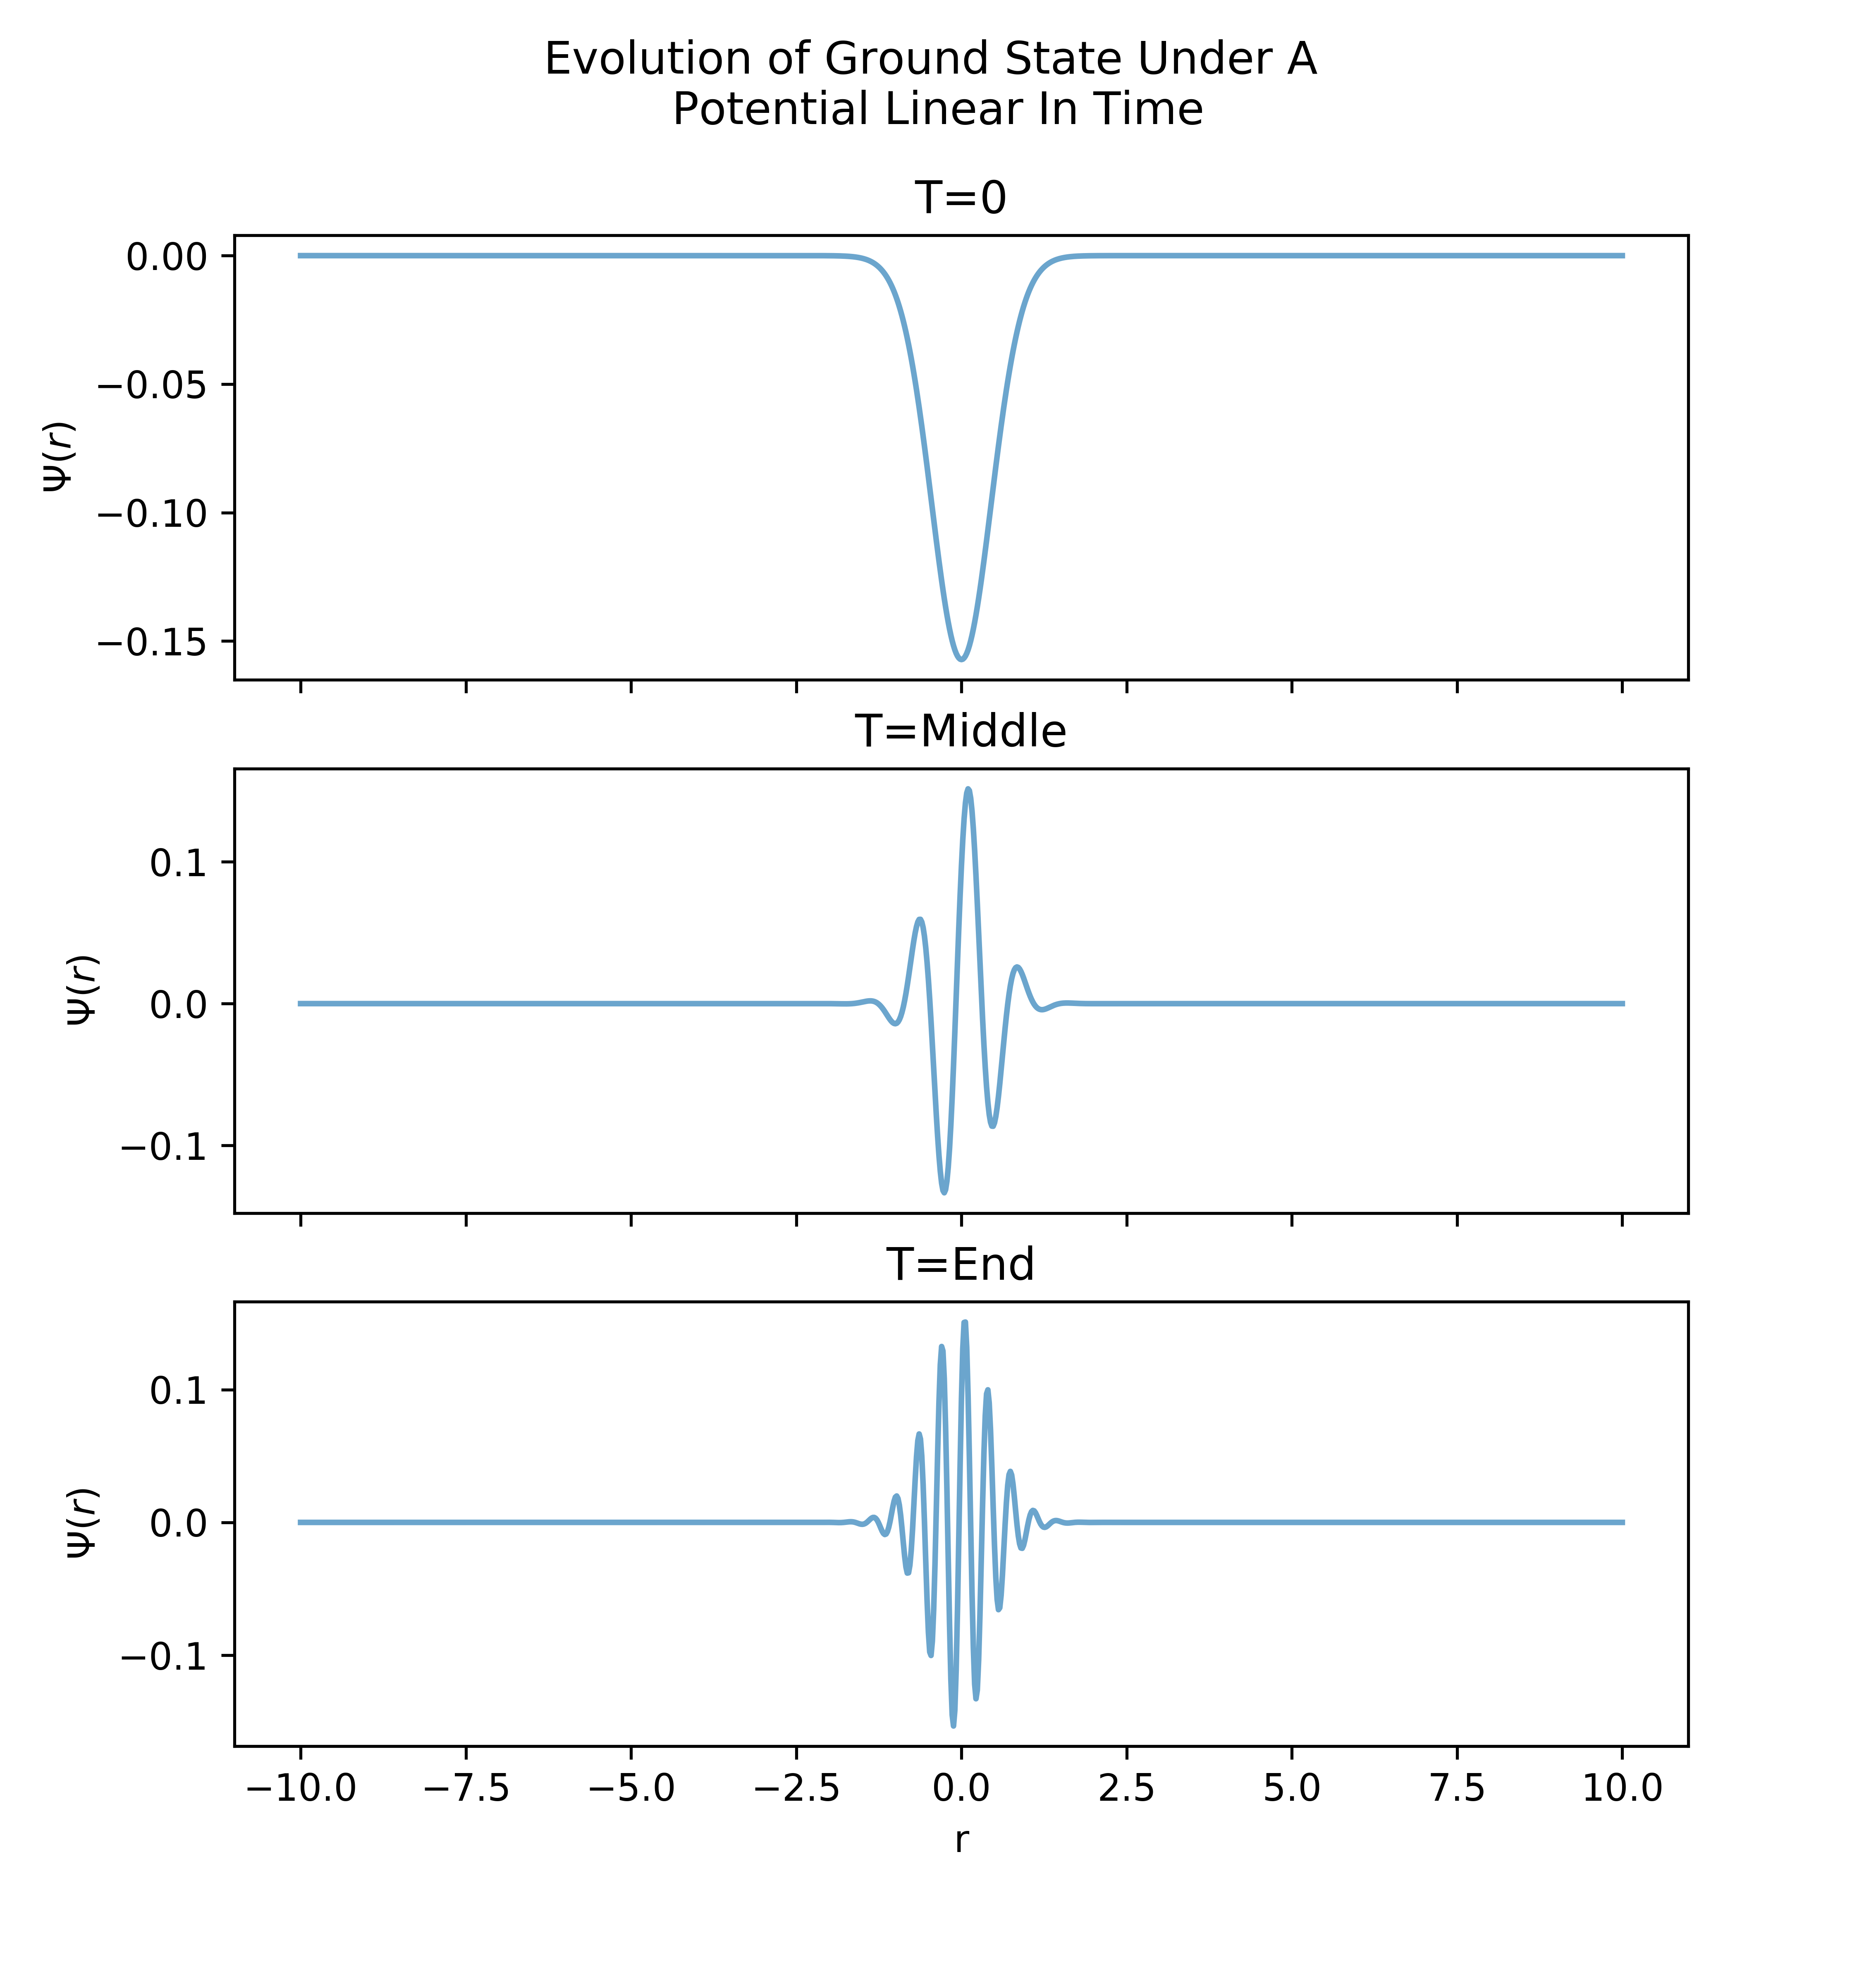
\includegraphics[width=\textwidth]{./GSLinTimeNEWwavefunction.png}
          \centering
          \caption{Effect of a linearly growing potential on wavefunction}
\end{figure}
From this figure, we see qualitatively that as time goes on the system is excited to higher and higher energies; shown through the increased numbers of turning points, and their relative magnitudes, indicating increasing contributions from higher energy eigenstates. Based on this, we can expect that the Ground State population will reduce over time as more and more eigenstates contribute and their contributions gain more and more weight. Figure 4.2, below, shows the decrease in the Ground State population over the same time interval:

\begin{figure}[H]
          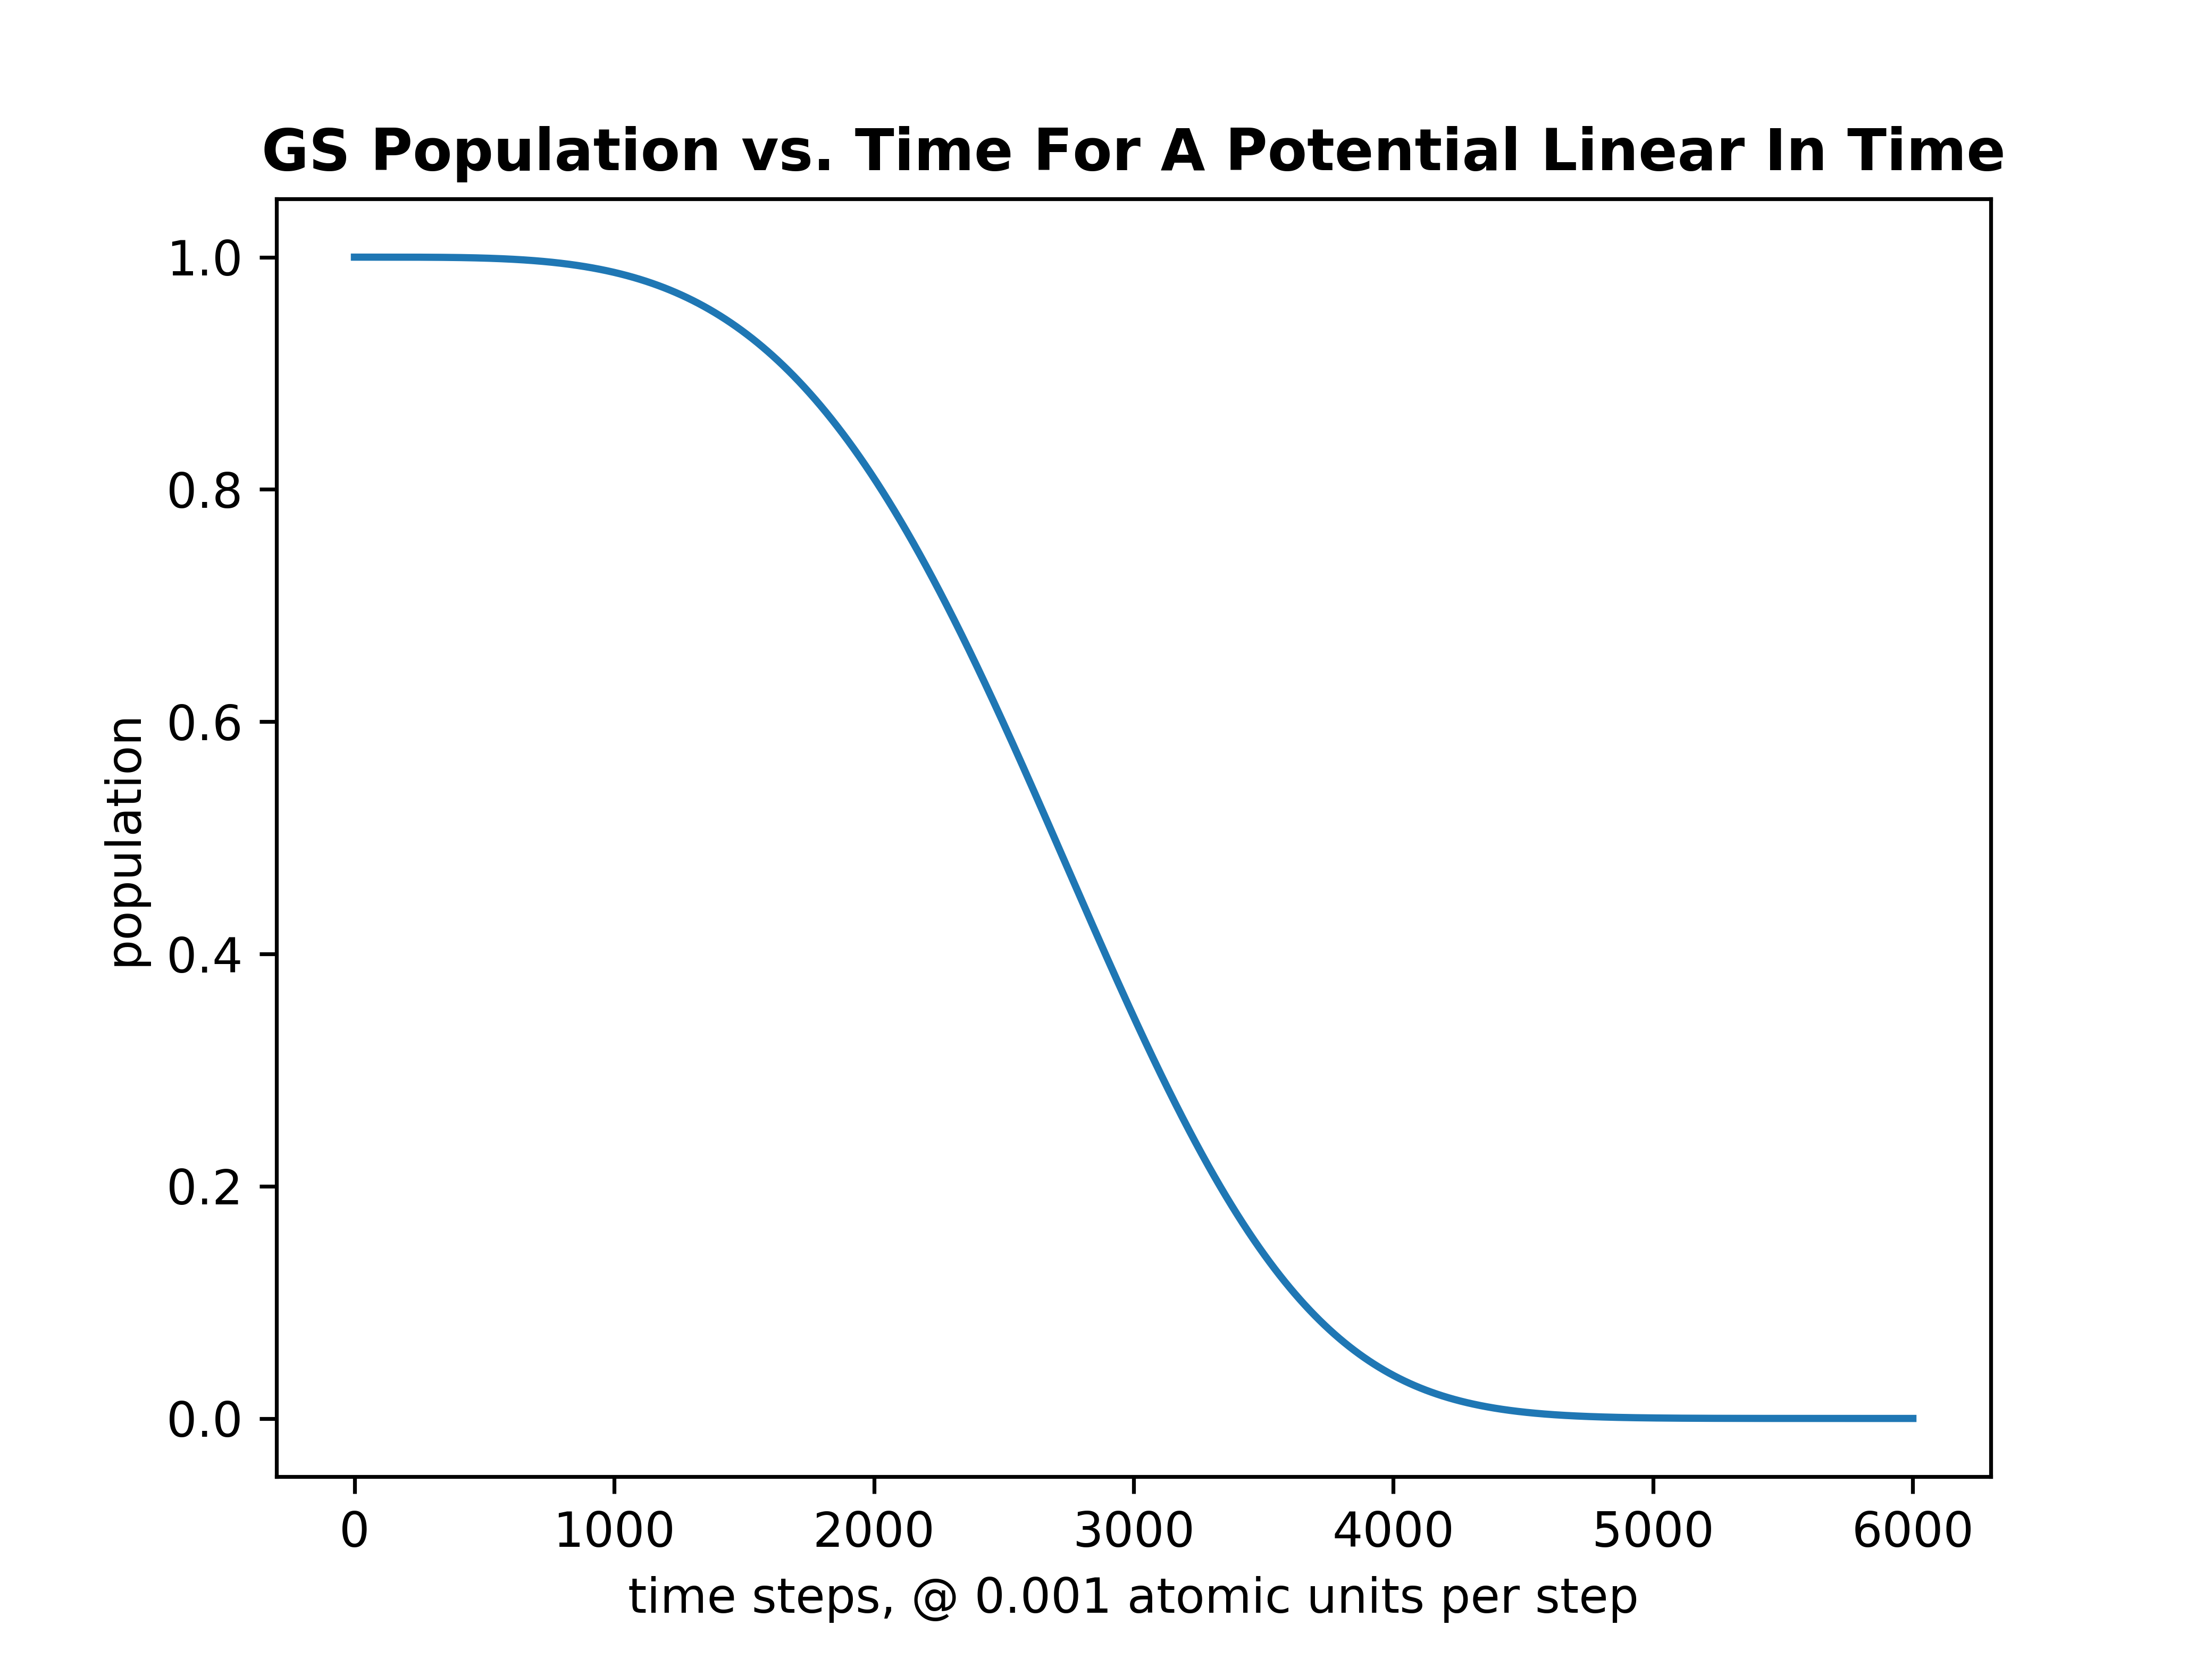
\includegraphics[width=\textwidth]{./GSLinTimeNEW.png}
          \centering
          \caption{Effect of a linearly growing potential on Ground State Population}
\end{figure}

\section{Gaussian Packet Potential}
In this section we investigate how our system would behave under the influence of a gaussian (with time) potential.

\subsection{Potential Description}
In this case, we build the external potential term as a gaussian packet w.r.t. time such that the centre of the packet (most intense part) occurs at 1 atomic unit of time, and the standard deviation of the packet is 0.25 atomic units of time. The intensity of the potential is controlled by a multiplicative factor, $\alpha$, giving the following expression for the external potential: 
$$
V_{\text{ext}} = \alpha \frac{4}{\sqrt{2\pi}}e^{-8\left(t-1\right)^{2}}\mathbf{r}
$$

As with the previous example, this extra potential term was added to the softcore potential, and the result used along the central diagonal of the Hamiltonian.

\subsection{Effect On State Evolution}

\begin{figure}[H]
          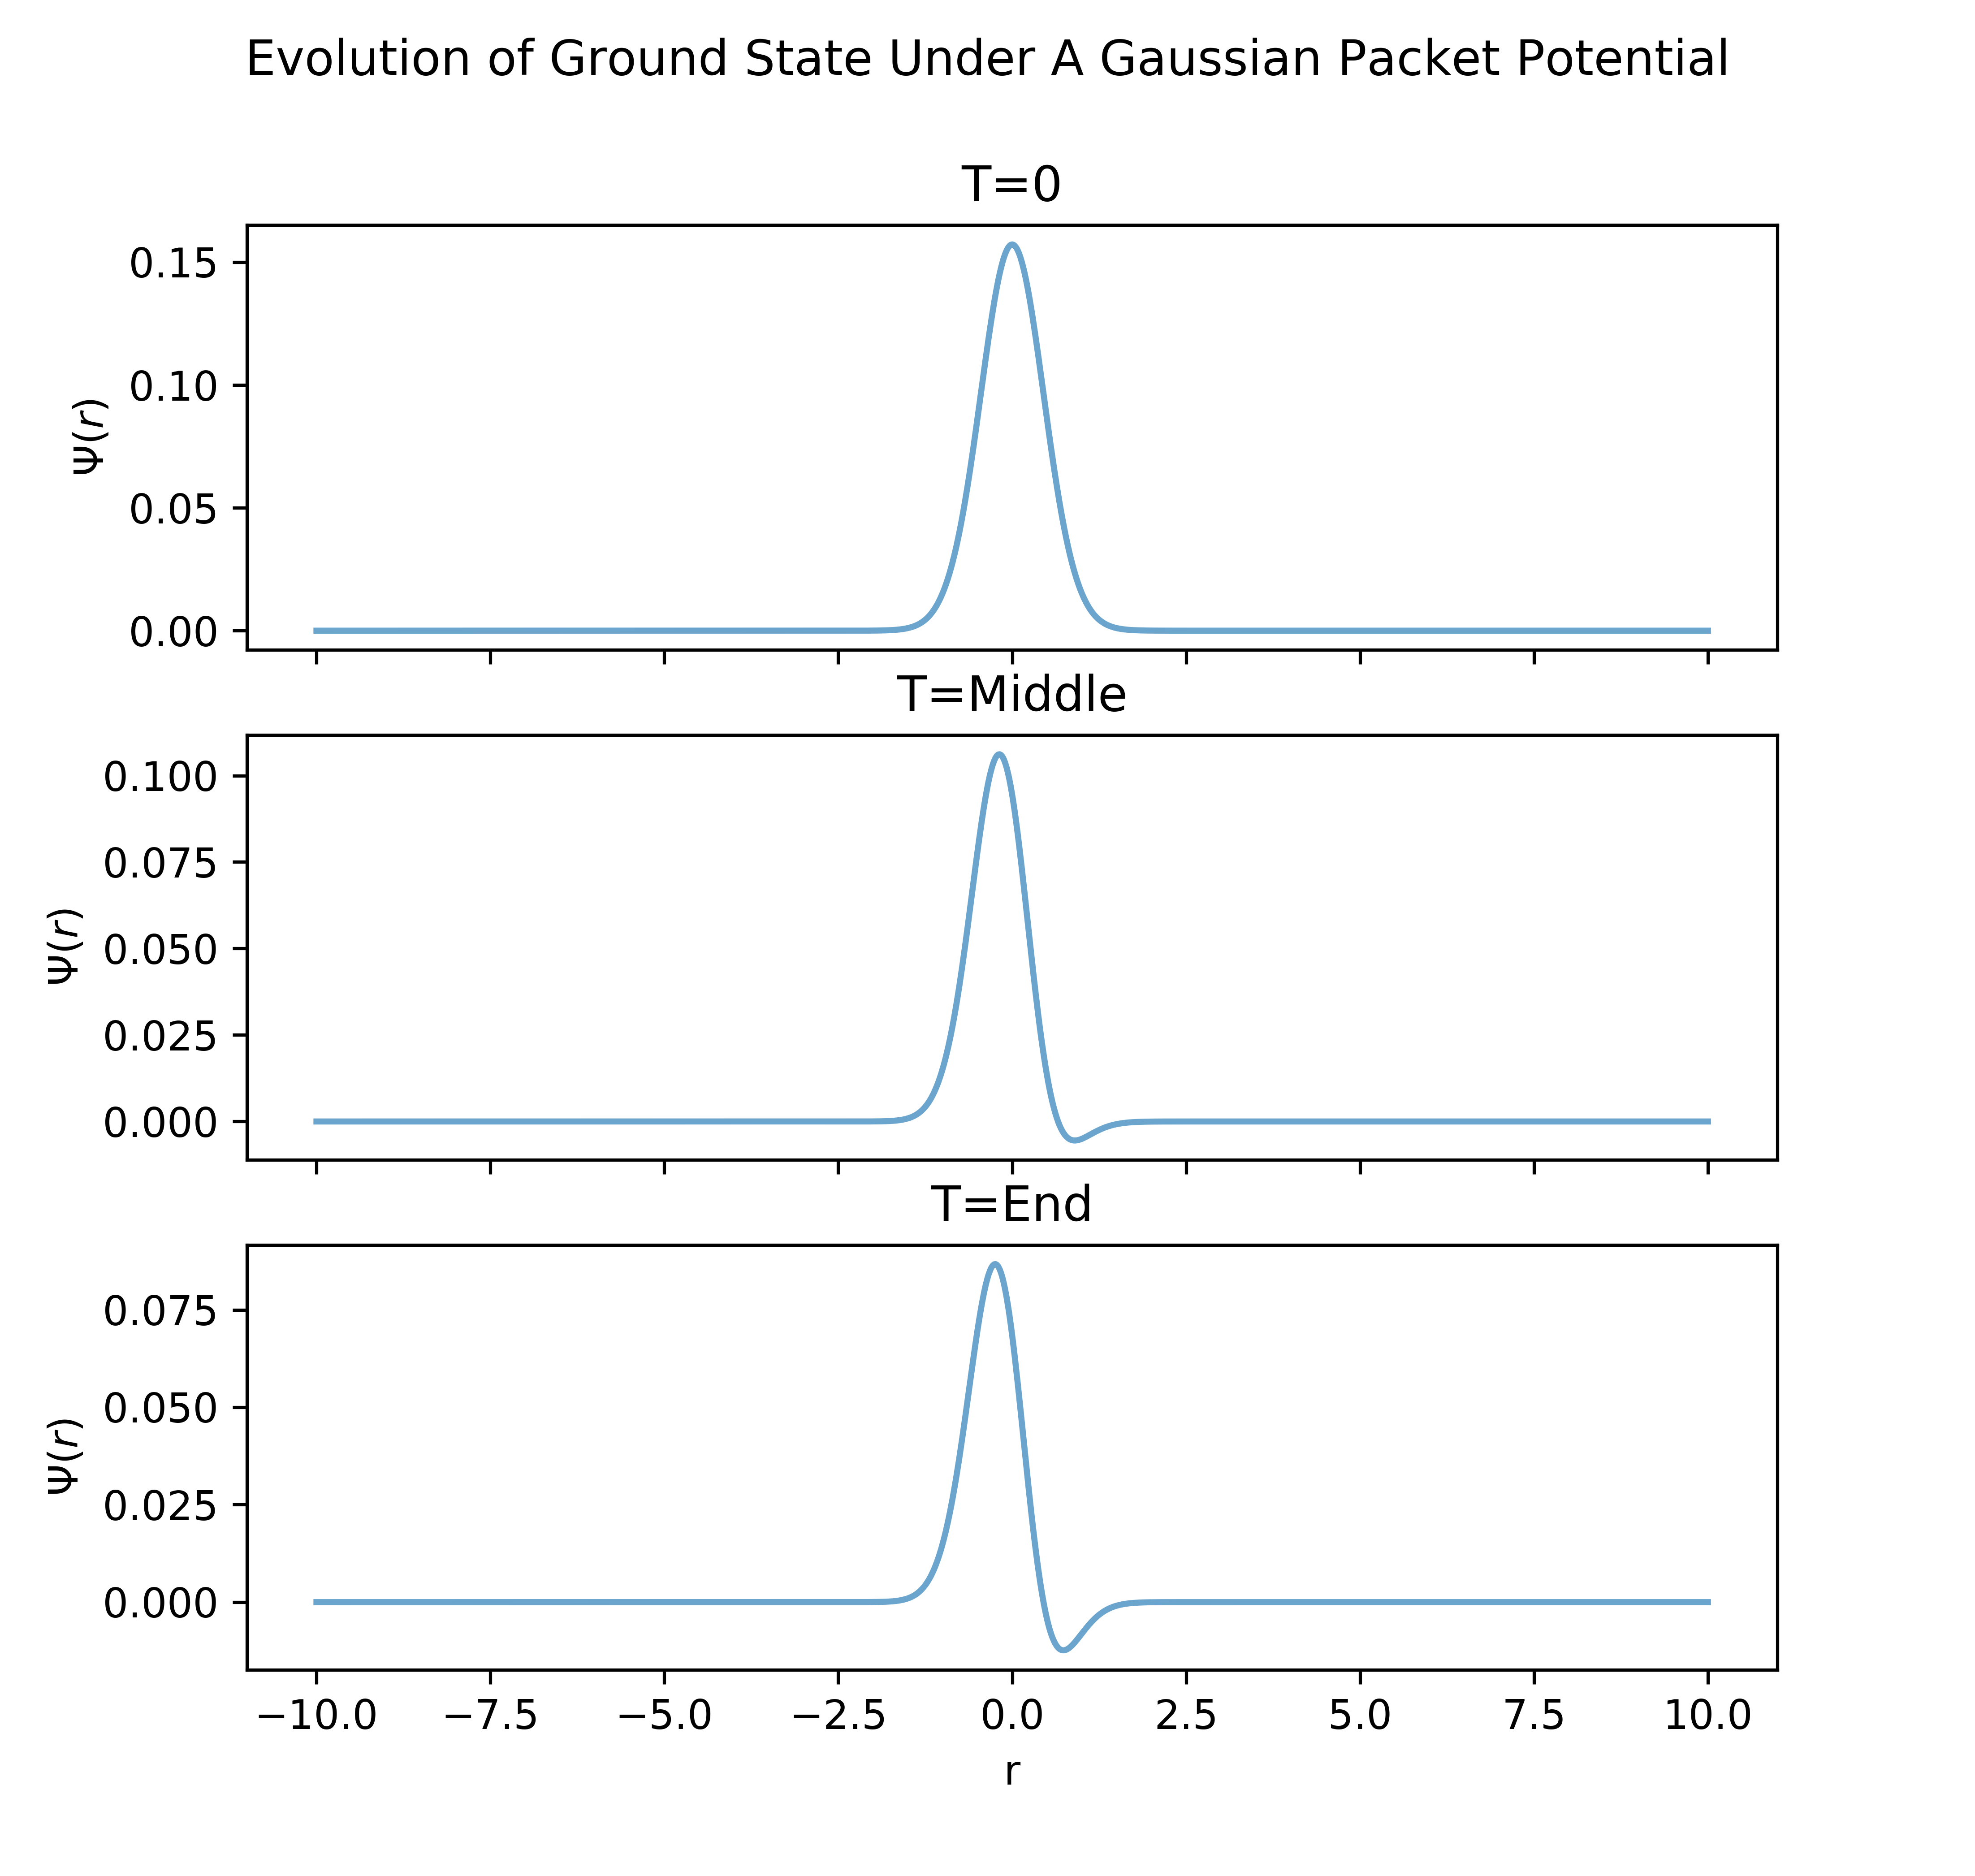
\includegraphics[width=\textwidth]{./GS1GaussianPacketNEWwavefunction.png}
          \centering
          \caption{Effect of Single Gaussian Packet on wavefunction}
\end{figure}

Figure 4.3, above, we see that almost all of a relatively small amount of energy is absorbed some time between the start and mid-point of the simulation (an interval of 3 atomic units of time), seen through the small additional turning point indicating a small contribution from the first excited state. There is very little change in shape between the mid-point and end of the simulation, indicating that there was very little incoming / outgoing energy in this time period.

The change to Ground State population was investigated over the same time interval, and the results shown in Figure 4.4, below:
\begin{figure}[H]
          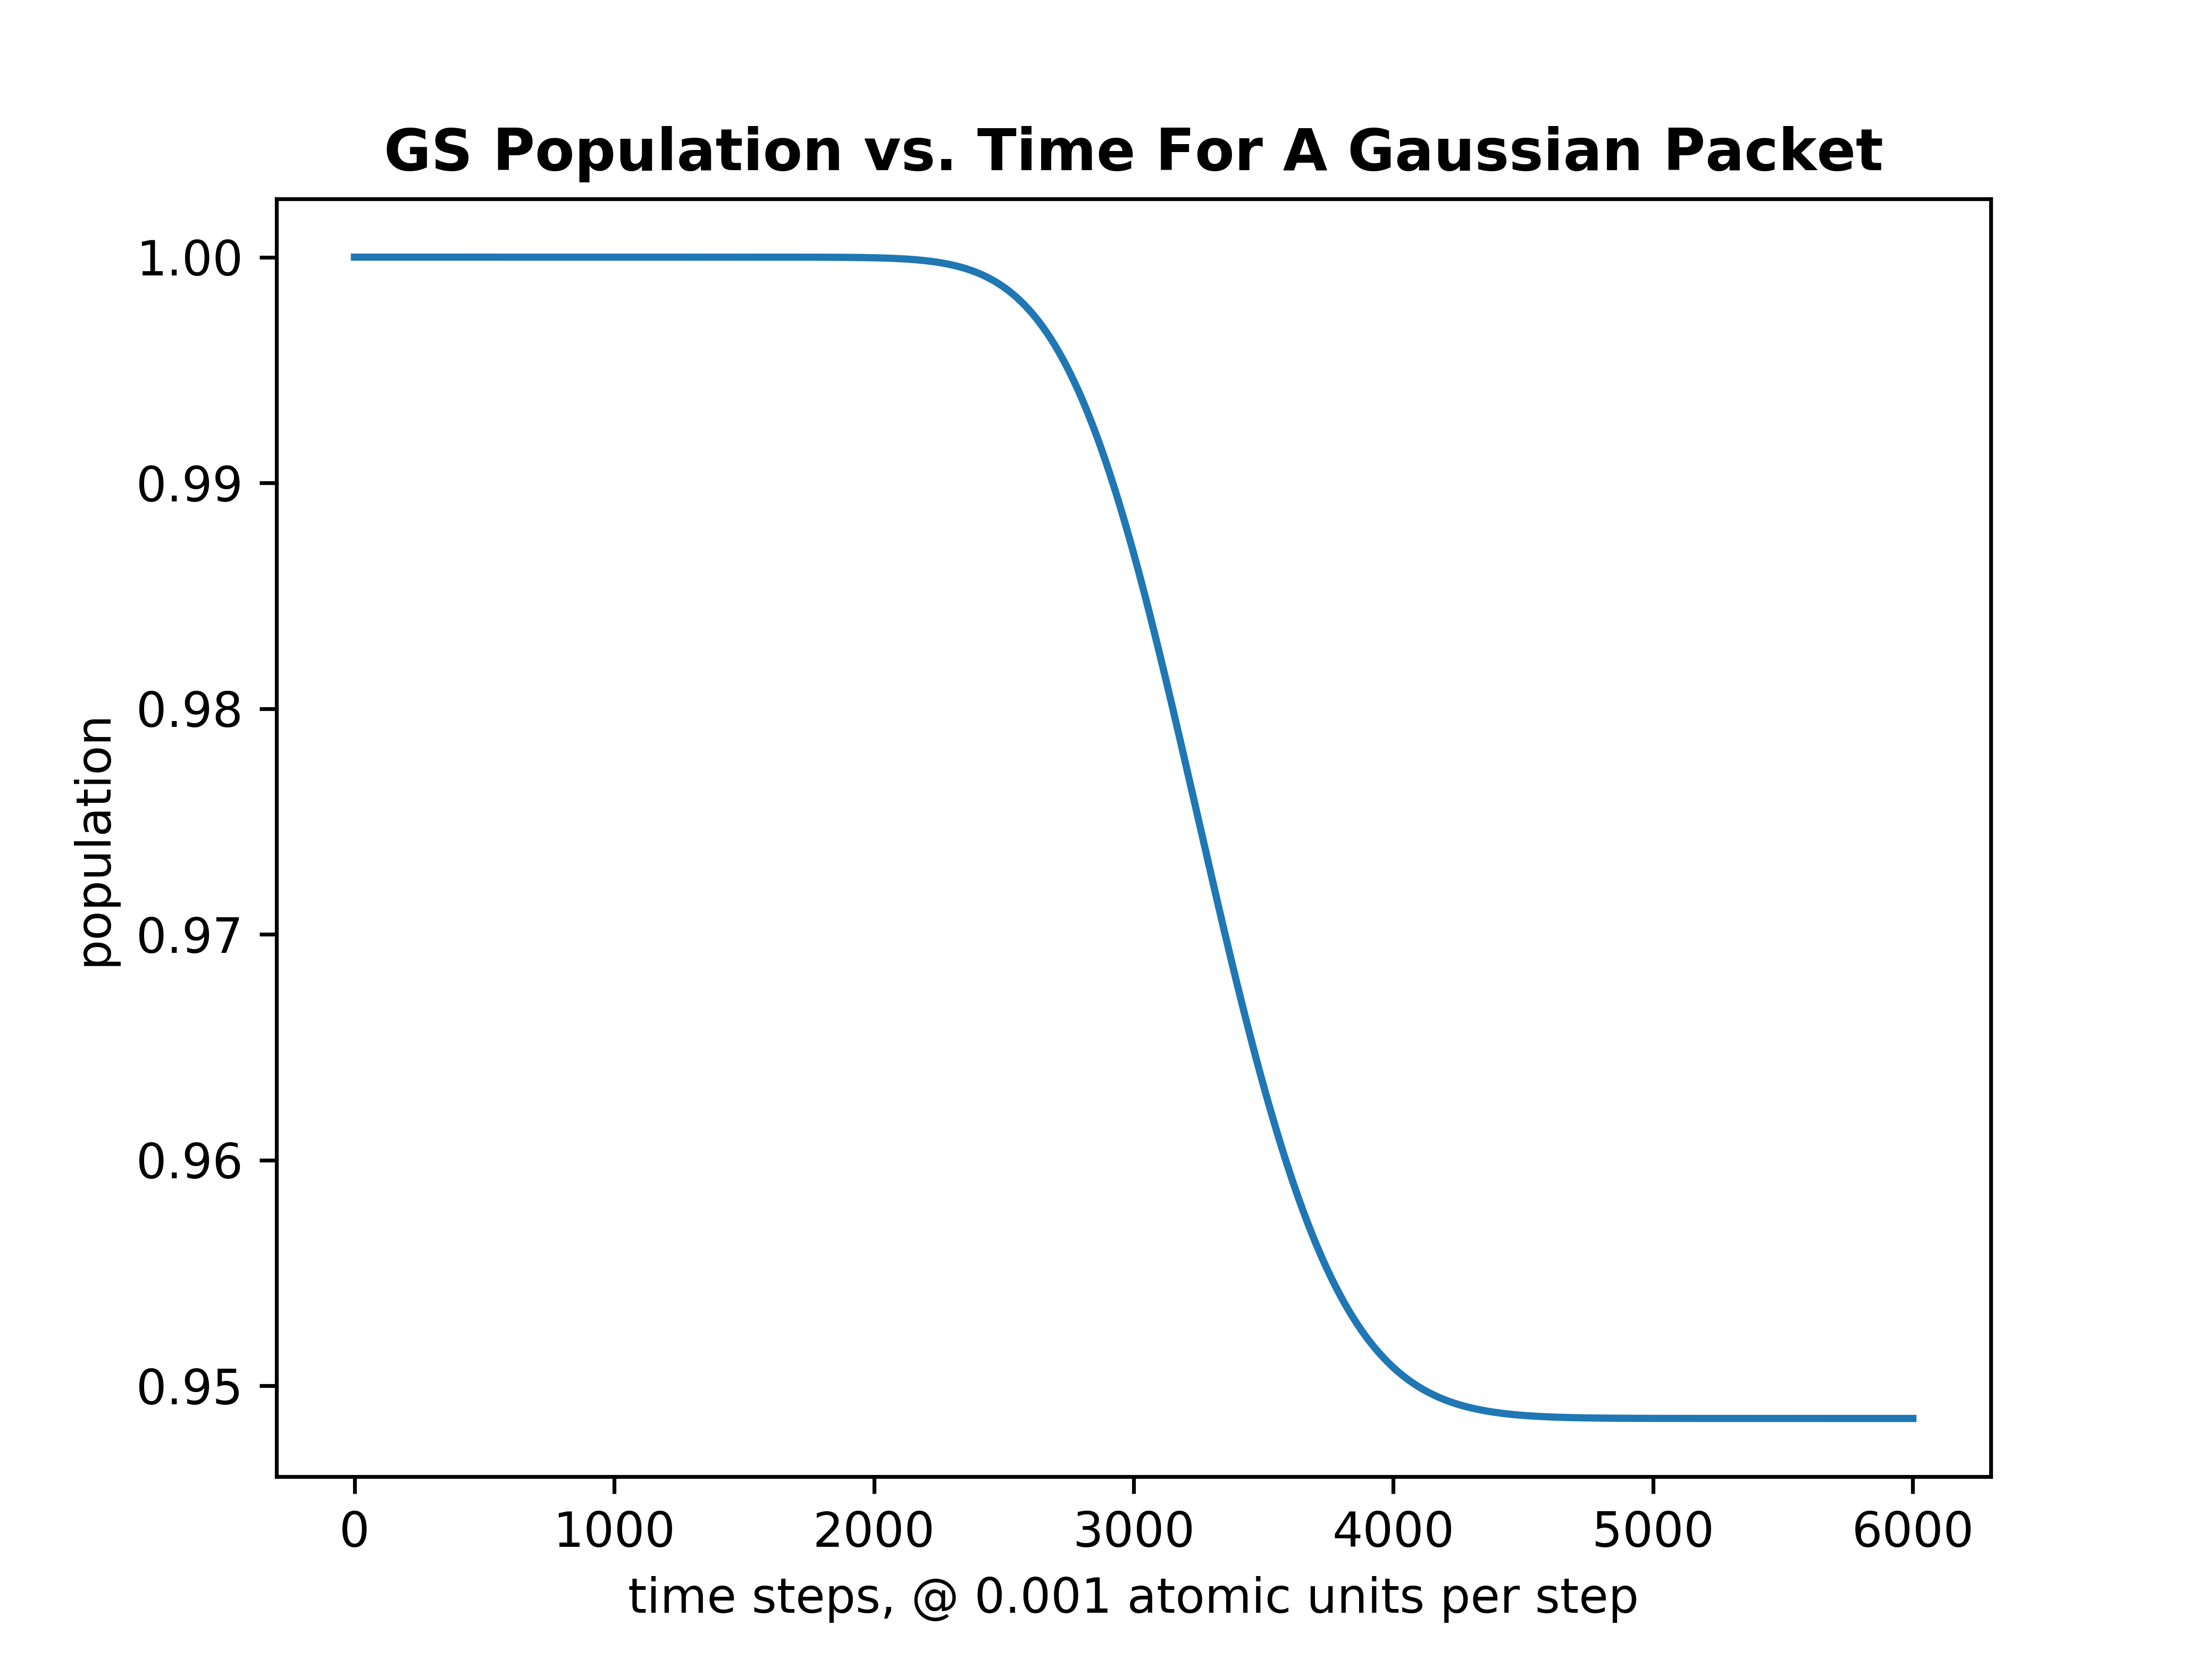
\includegraphics[width=\textwidth]{./GS1GaussianPacketNEW.png}
          \centering
          \caption{Effect of Gaussian Packet on GS population}
\end{figure}

This graph shows that between around 0.5 and 1.5 atomic units of time into the simulation, the wavefunction is rapidly excited; losing 5\% of the population by 1.5 atomic units of time. Adter this initial loss, the population stays steadily at around 95\% for the rest of the simulation, indicating no further change to its energy.

\section{Multiple Gaussian Packets}

We investigate the effects on our system of subjecting it to a series of gaussian potentials over the course of the simulation. 

\subsection{Potential Description}
The external potential used in this simulation is similar to the one used in the previous simulation, but with three added to the softcore potential to form the total potential term rather than one. Additionally, two of the packets have their centres shifted to occur at 3 and 5 atomic units of time.

\subsection{Effect On State Evolution}
The graphs in the figure below describe the evolution of the system as it absorbs energy from repeated gaussian potentials. This differs from the previous investigation of a single packet in that the end result is a system with noticeably higher contributions from excited states than previously, indicating that the system has absorbed more energy. Additionally, the wavefunction of the system at the end shows higher exctited state contributions than in the middle of the simulation - indicating that energy is absorbed both before and after the mid-point of the simulation, matching expectations as the packets were staggered to be centred around $\frac{1}{6}, \frac{3}{6}, \text{ and }\frac{5}{6}$ of the simulation.
\begin{figure}[H]
          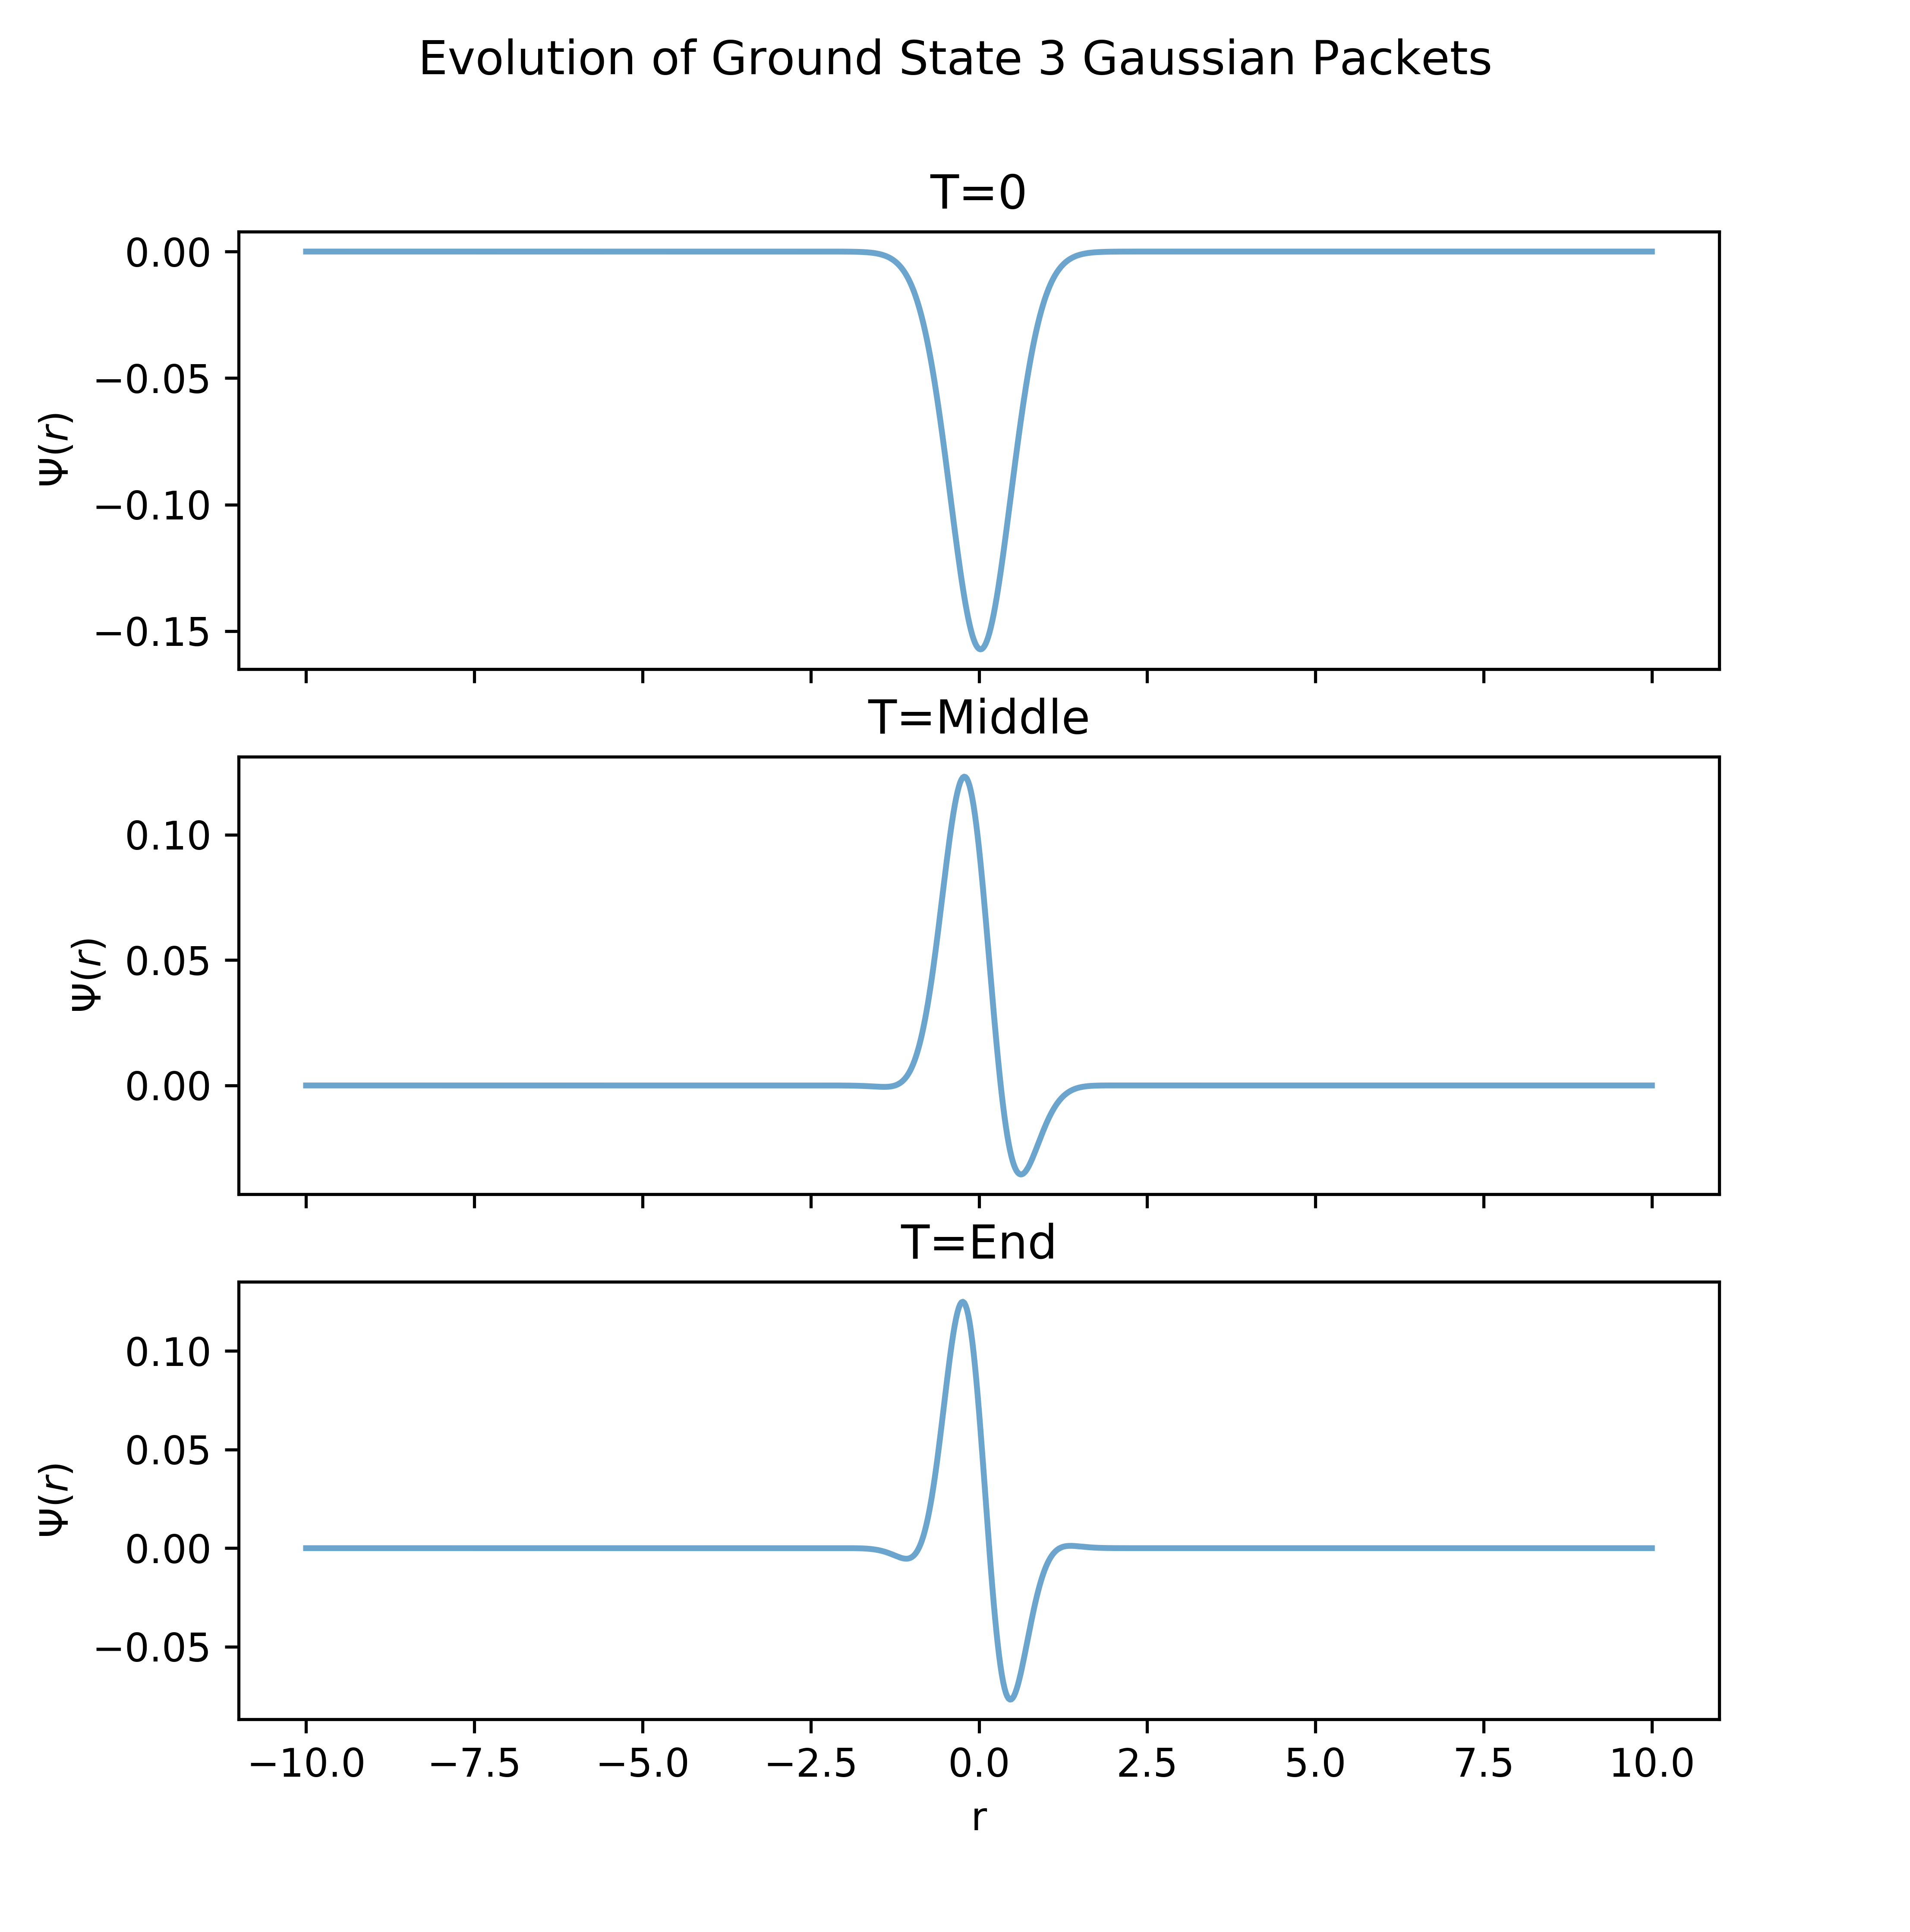
\includegraphics[width=\textwidth]{./GS3GaussianPacketNEWwavefunction.png}
          \centering
          \caption{Effect of 3 Gaussian Packets on wavefunction}
\end{figure}

The Ground State population was also investigated, with the results shown in Figure 4.6 below, and we can see that there are three distinct drops in population - centred around 1, 3, and 5 atomic units of time; matching when we placed the maxima of the laser pulses. Additionally, we can see that the repeated laser pulses led to a higher overall drop in Ground State population by the end of the simulation, matching the analysis of the evolution of the wavefunction where we noticed higher contributions from excited states than with the single laser pulse.
\begin{figure}[H]
          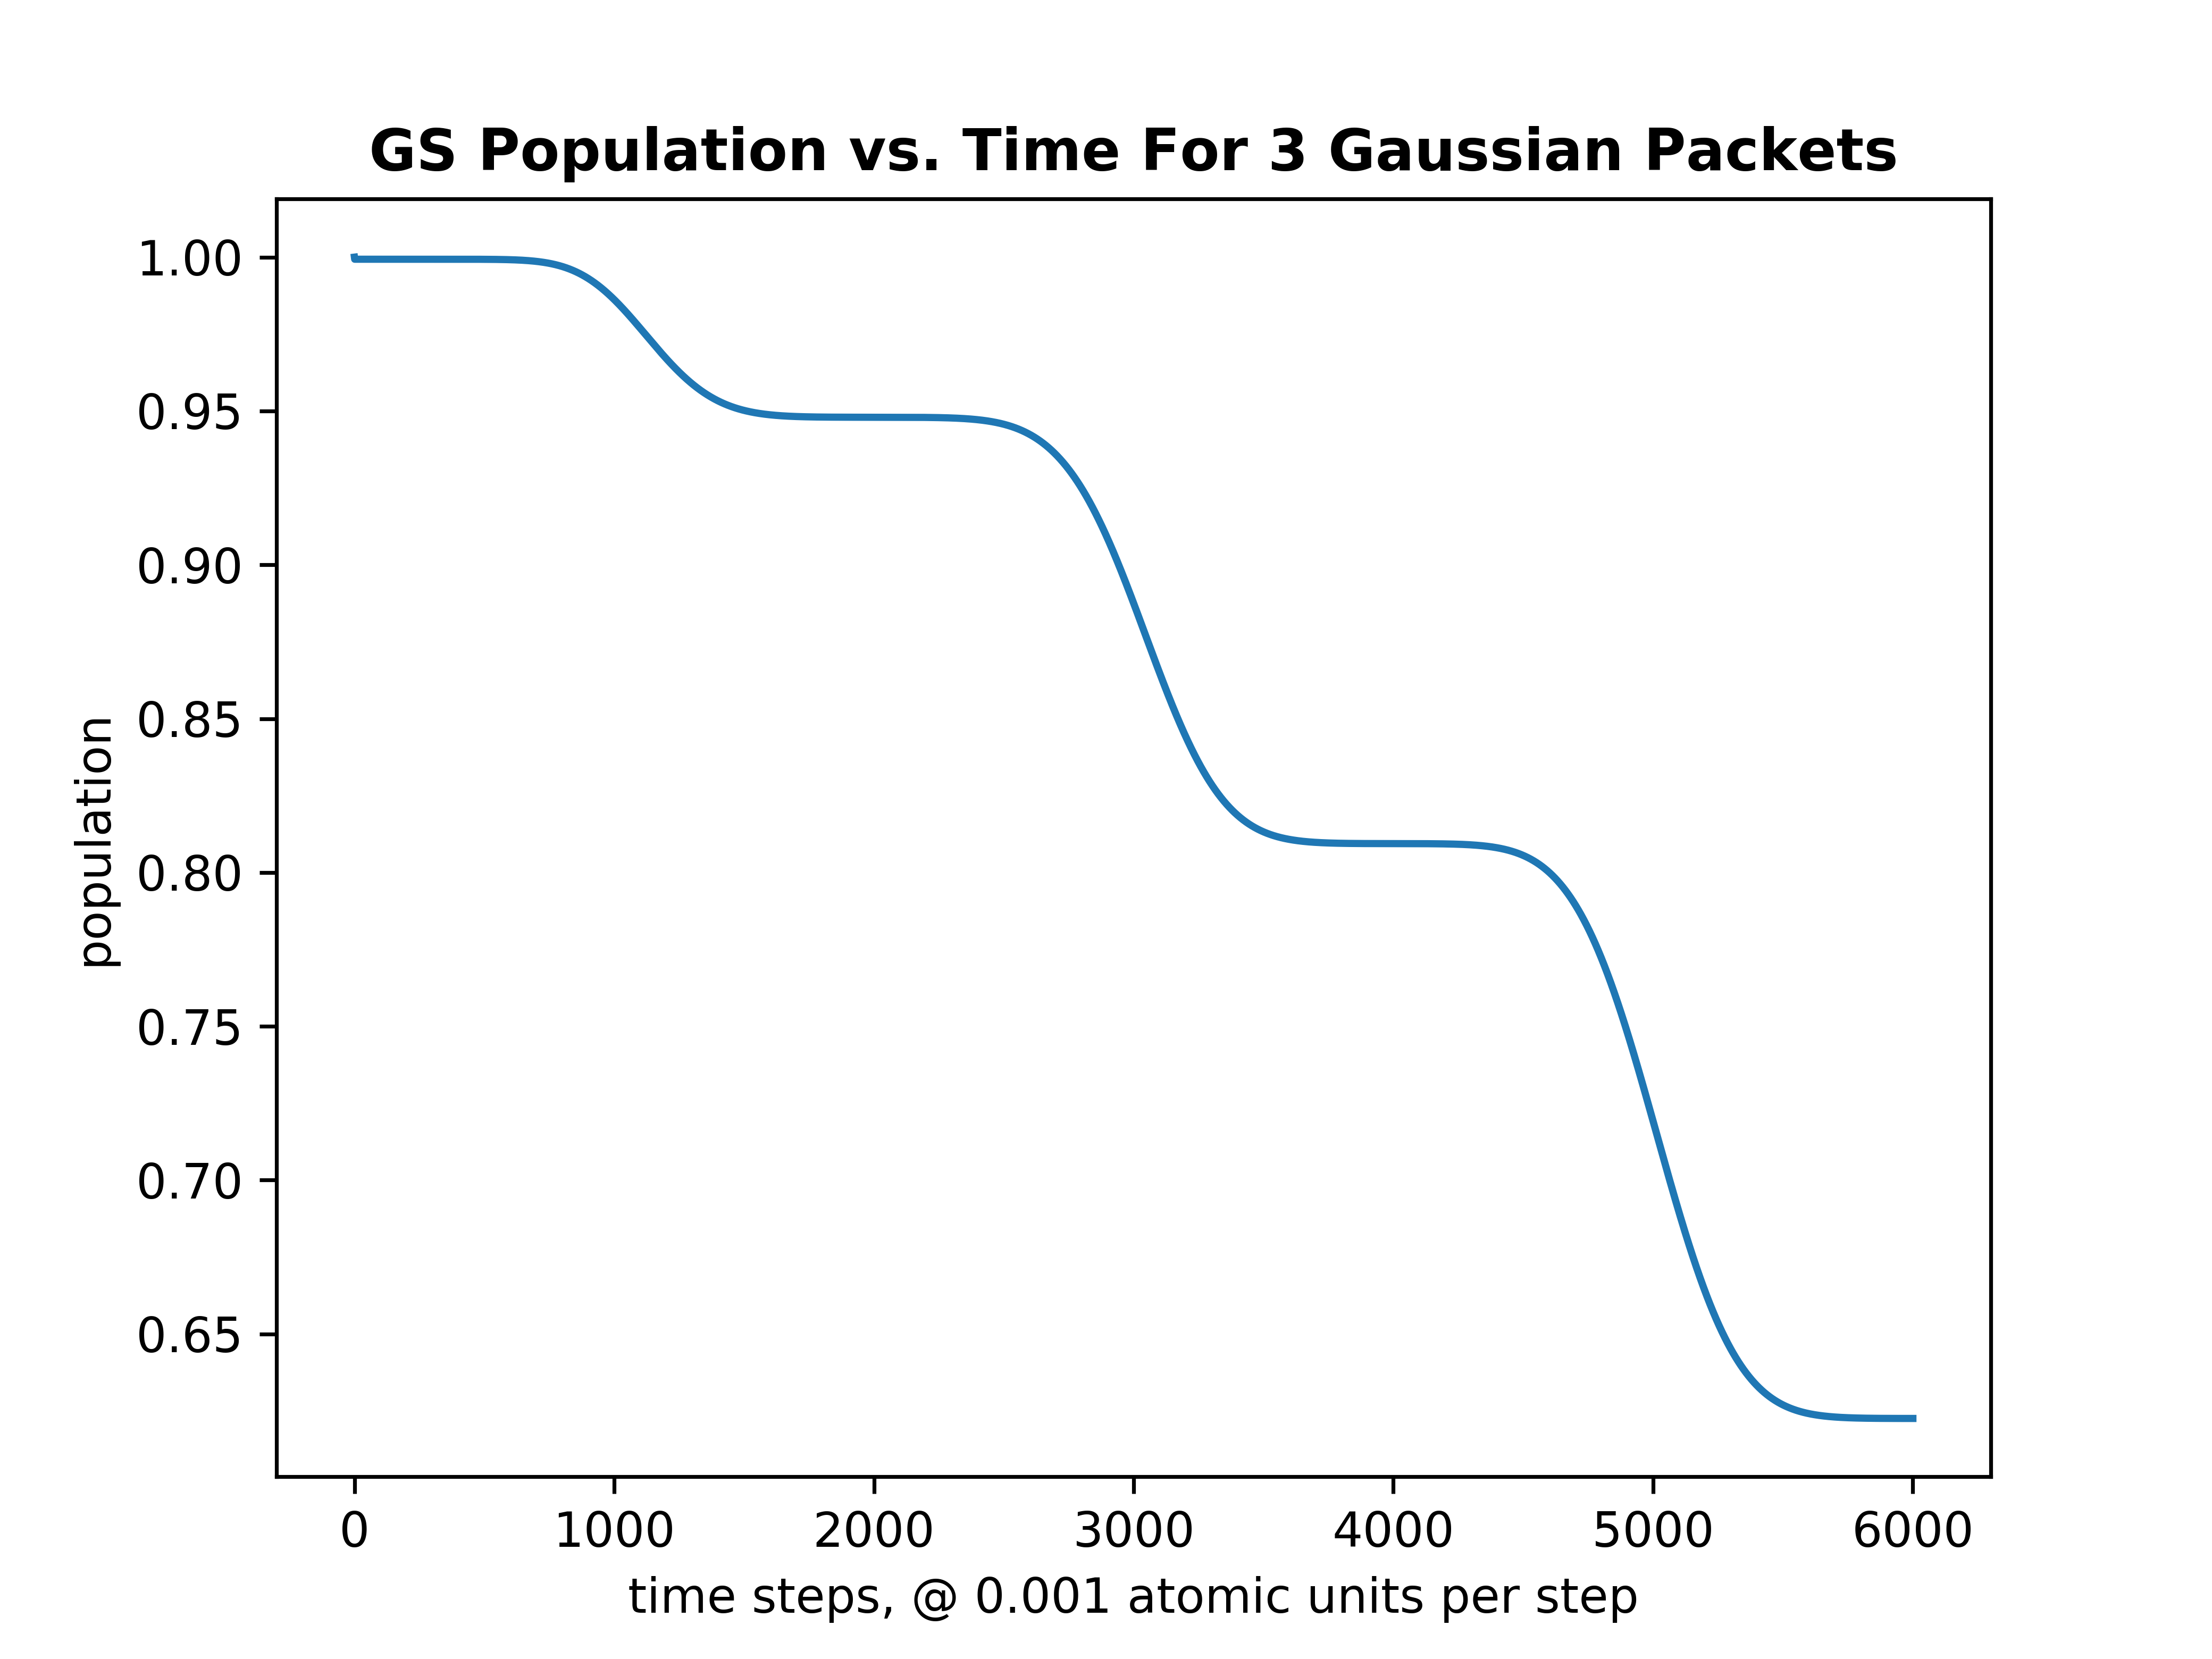
\includegraphics[width=\textwidth]{./GS3GaussianPacketNEW.png}
          \centering
          \caption{Effect of 3 Gaussian Packets on GS population}
\end{figure}

\section{Simulated Laser Pulse}

Here we model a Laser pulse interacting with our system using a potential built by encapsulating a sinusoidal wave within a gaussian packet to model our Laser pulse. Mathematically, this potential is described by;
$$
V_{\text{ext}} = \alpha \frac{2}{\sqrt{2\pi}}e^{-2\left(t-3\right)^{2}}\mathbf{r}\ \text{sin}\left(\omega t\right),
$$
where $\omega$ is the frequency of the sinusoidal term and $\alpha$ is a multiplicative factor controlling the intensity.

The figure below describes the field strength of this potential over the course of the simulation, and qualitatively demonstrates its similarity to a laser pulse potential:
\begin{figure}[H]
          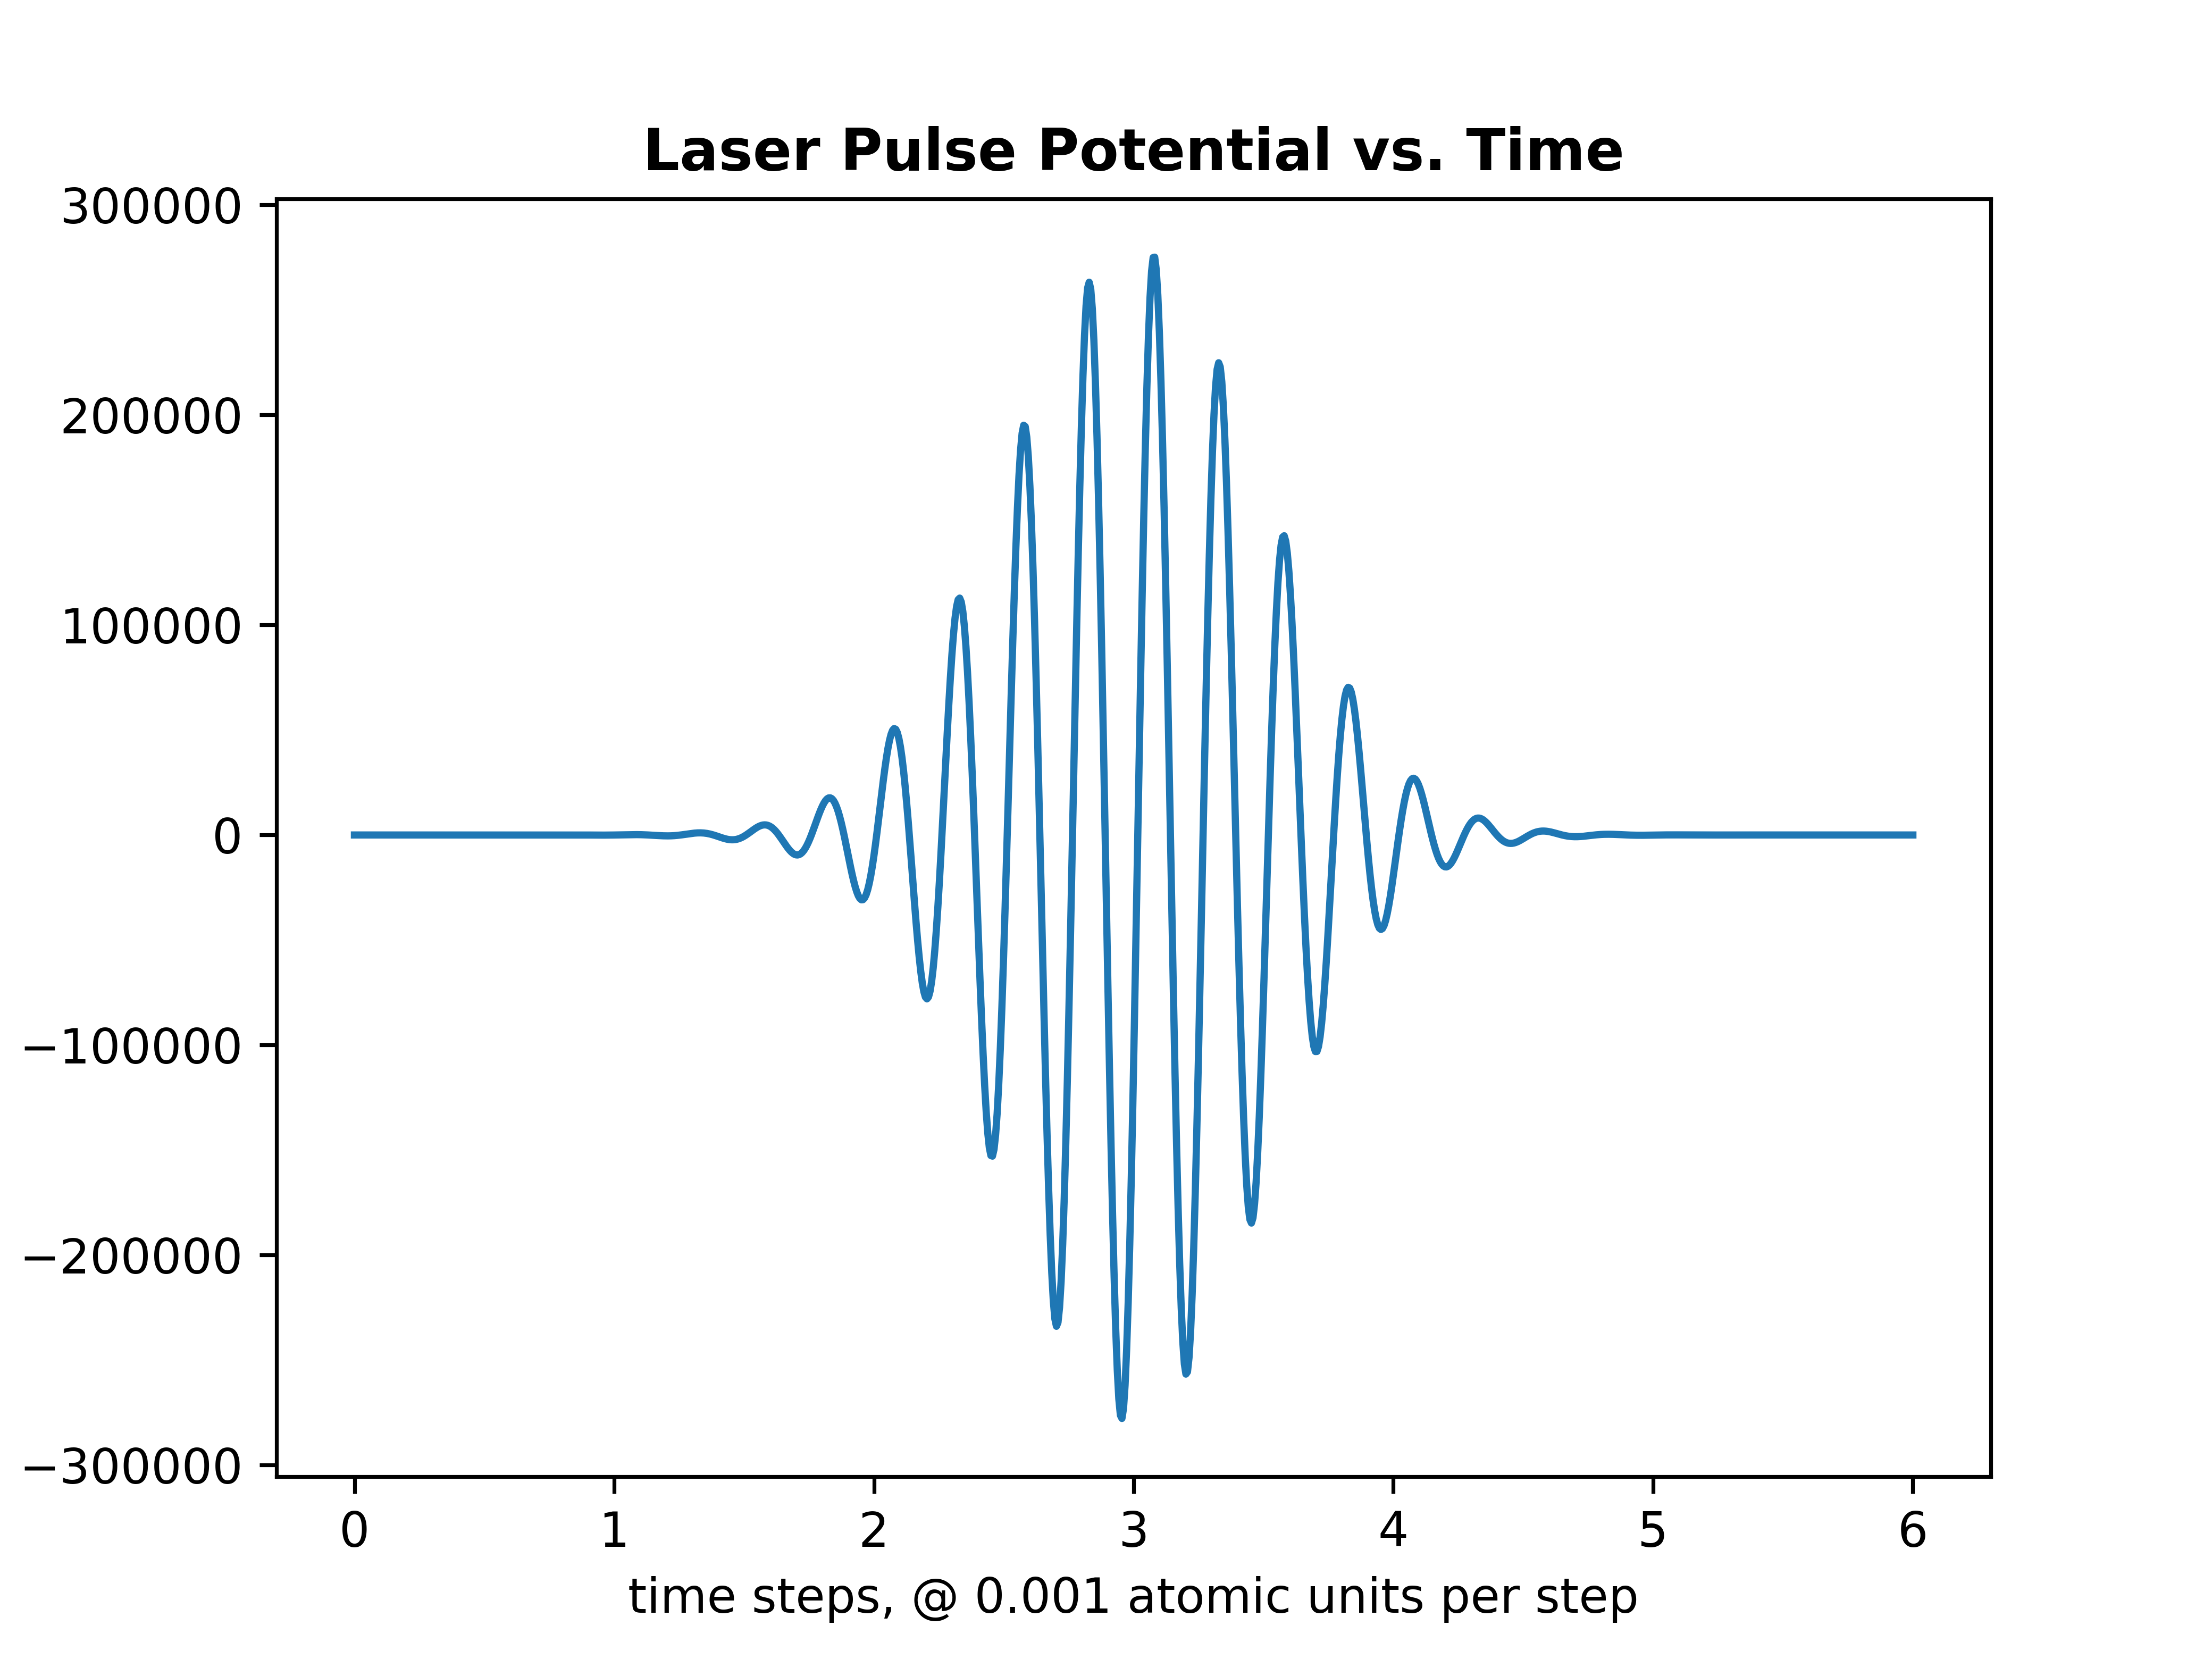
\includegraphics[width=\textwidth]{./LaserPulseNEWPotential.png}
          \centering
          \caption{Potential Field Strength Over Time For Laser Pulse}
\end{figure}

Upon interacting with our system, rapid gains and losses of energy are made as the direction of the potential cycles. The following figure demonstrates this effect;
\begin{figure}[H]
          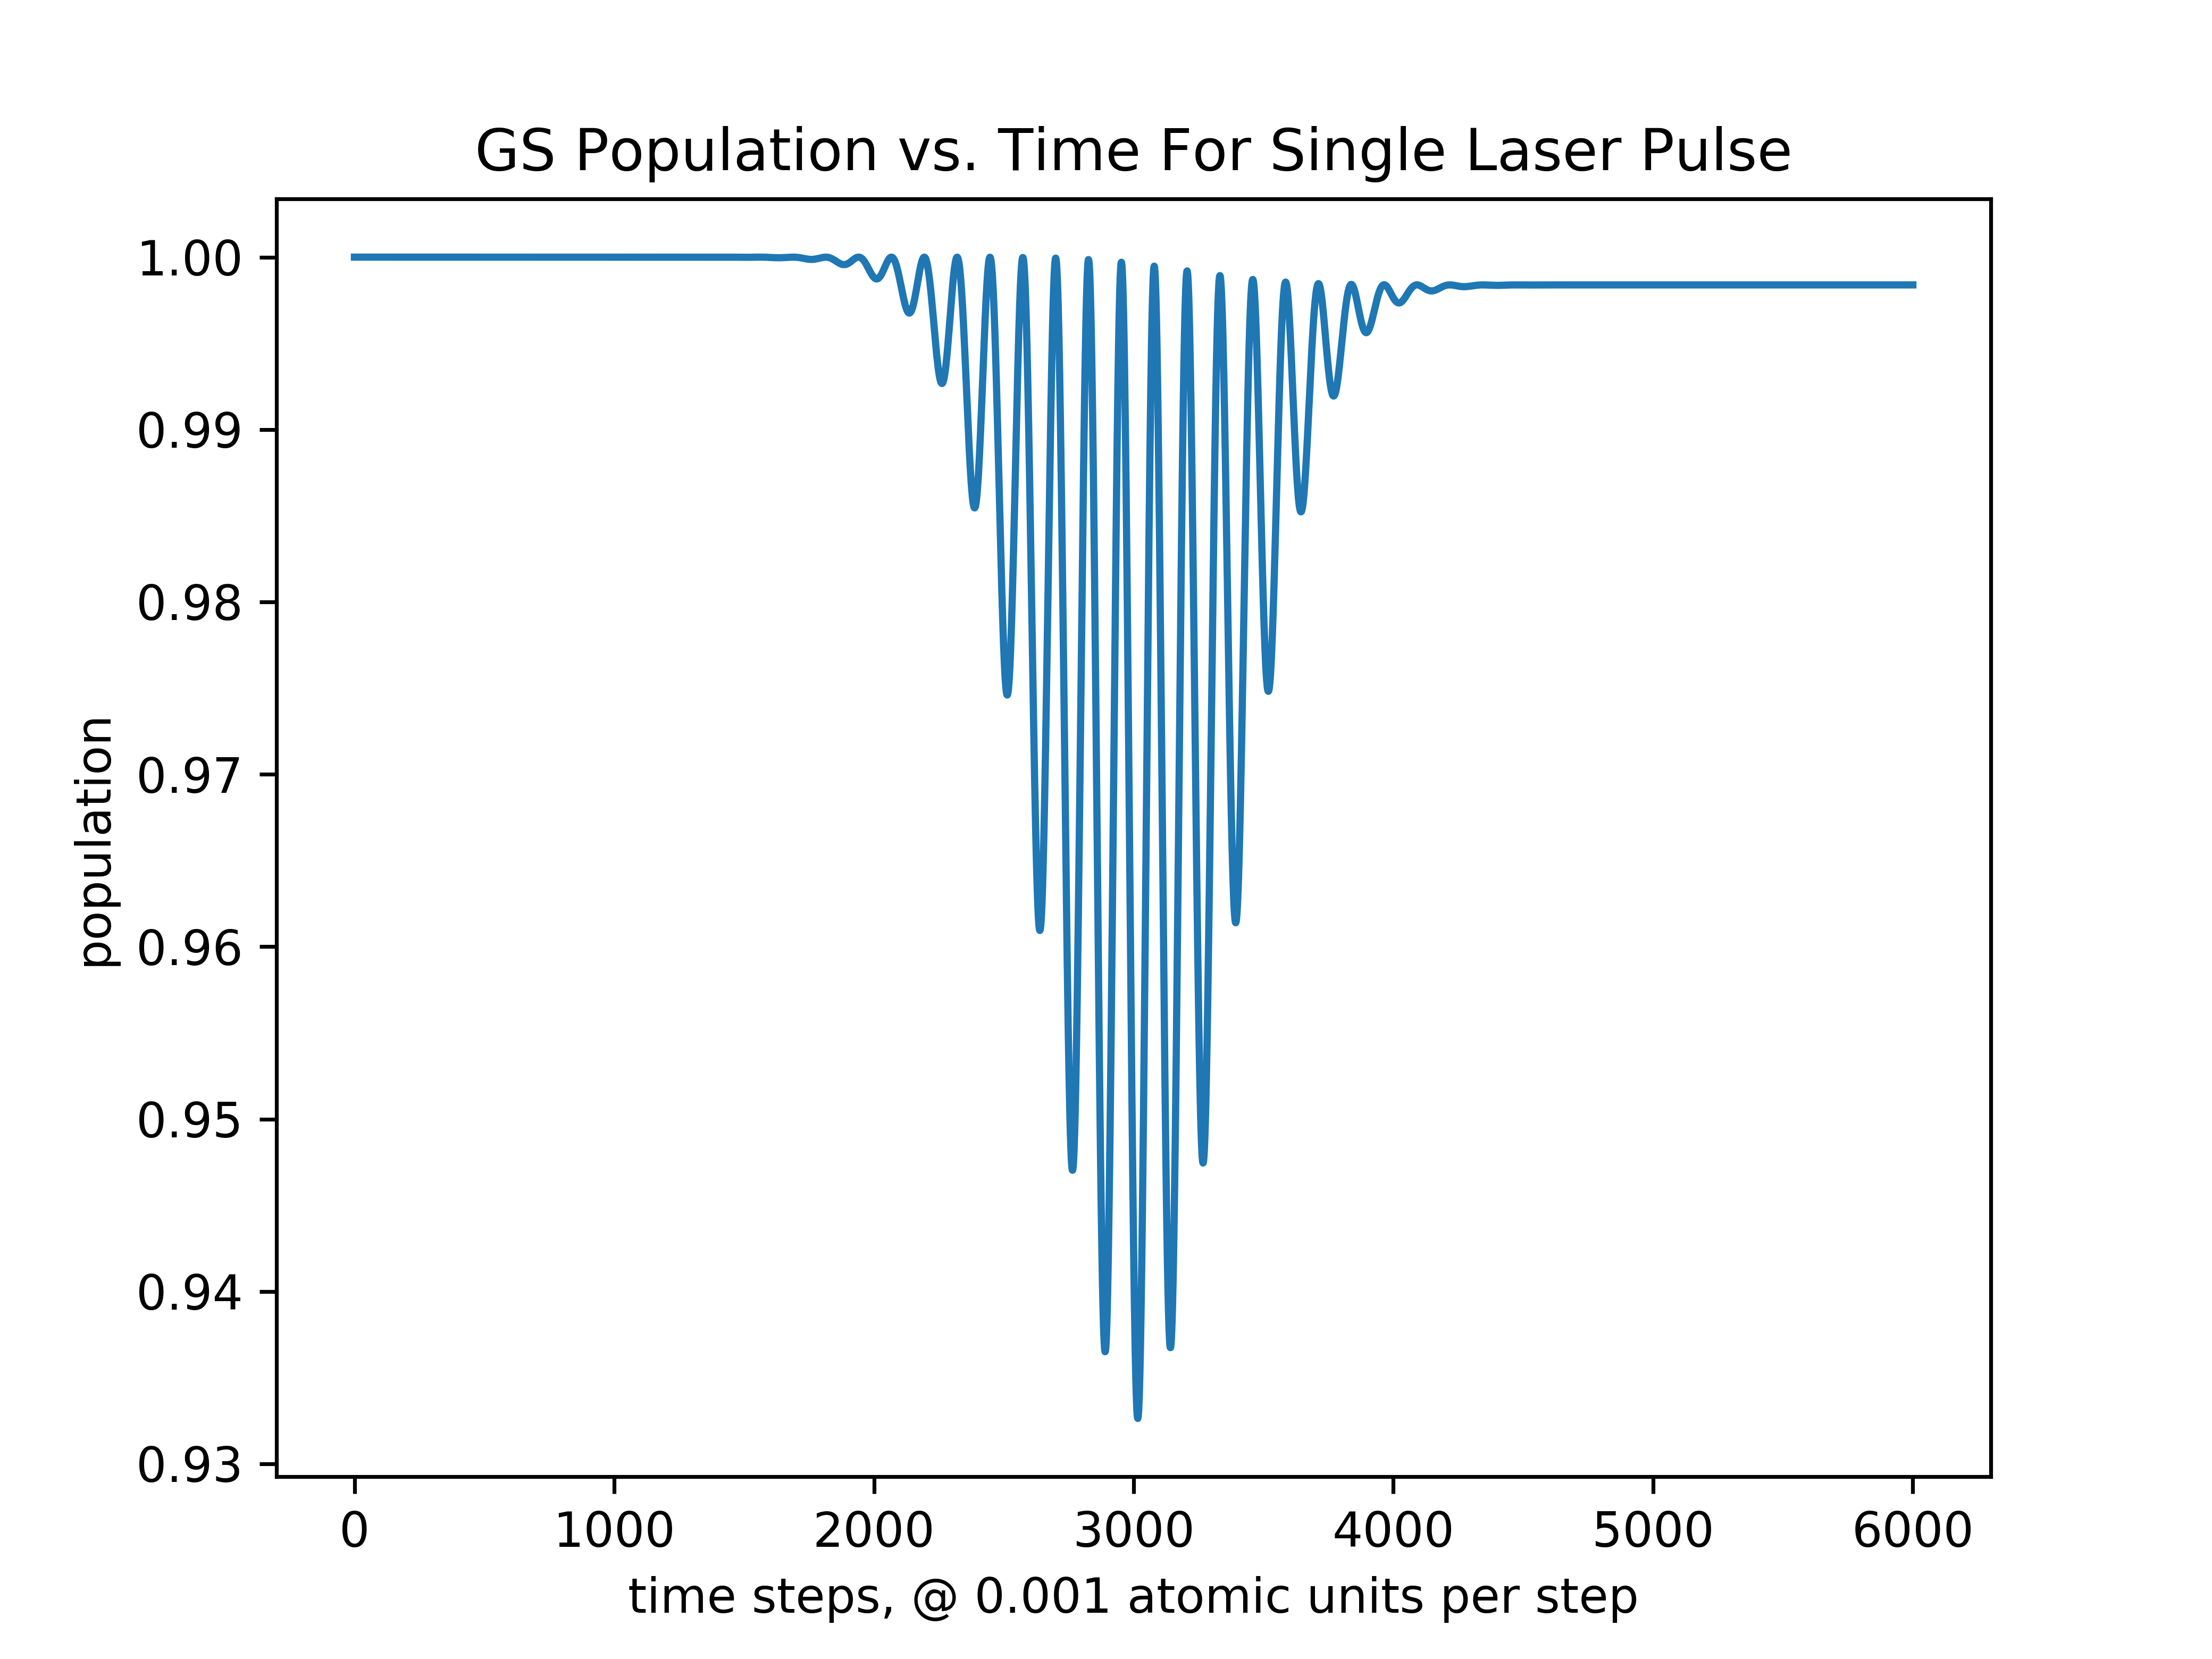
\includegraphics[width=\textwidth]{./GSSingleLaserPulseNEW.png}
          \centering
          \caption{Effect of Simulated Laser Pulse on GS population}
\end{figure}

Here we see that the wavefunction, initially entirely in the ground state, continuously gains and loses population in higher excited states as the pulse interacts - with the magnitudes of these gains and losses scaling with the magnitude of the gaussian packet enveloping the pulse. Additionally we see that almost, but not all of, the population is retained at the end of the pulse; leaving a small amount ($\simeq 1\%$) of the population in higher excited states.

%----------------------------------------------------------------------------------------
